\section{Descrição}

O sistema em si (sem contar os periféricos), é formado pelo circuito que realiza os cálculos relacionados a regressão linear 
[linear regression.vhd], pela memória [ram.vhd] e pela máquina de estados [linear regression fsm.vhd] que controla a regressão linear.
Conectados a esse sistema, estão os periféricos que são um teclado numérico para a entrada de dados e um monitor 
que mostra os dados sendo digitados, os pontos no gráfico e por fim a reta que vem da regressão linear.

\subsection{Diagrama de Blocos}

    \begin{figure} [H] 
        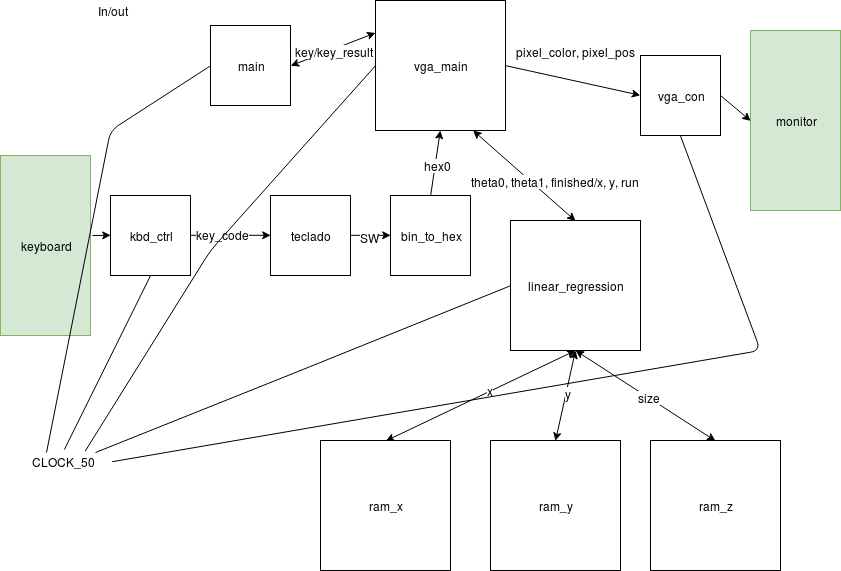
\includegraphics[width=\textwidth]{blockdiagram}
        \caption{Diagrama de Blocos}
        \label{fig:blockdiagram}
    \end{figure}

\subsection{Implementação}

A implementação de [linear regression.vhd] consiste em realizar as fórmulas referidas na parte teórica. 

\subsubsection{Pontos Fixos}

Para uma regressão linear precisa, é necessário a utilização de casas decimais nas contas, para evitar a 
necessidade de implementar representação por ponto flutuante, que é complexa, utilizamos um ponto fixo:
 Um vetor, guardando a parte decimal numa metade, e a parte fracionária em outra. 
Tal escolha facilitou as operações, e reduziu pouco a eficiência.

\subsubsection{Memória}

O algoritmo usa 3 memórias de 256 palavras, com 8 bytes cada, a motivação para isso, 
é que não há necessidade de um conjunto muito vasto de dados, porém, com 8 bytes, é possível alcançar uma boa precisão para cálculos.
As memórias são usadas para armazenar:

\begin{enumerate}
    \item os valores em um vetor de entradas
    \item os valores em um vetor de saída
    \item outros dados (como tamanho do vetor)
\end{enumerate}

\subsubsection{Máquina de Estados}

    \begin{figure} [H] 
        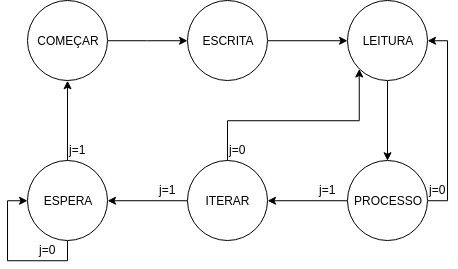
\includegraphics[width=\textwidth]{sm-linreg}
        \caption{Máquina de Estados - Regressão Linear}
        \label{fig:sm-linreg}
    \end{figure}

A máquina de estados que controla a regressão linear está sincronizada com a borda de descida do [CLOCK 50], ao contrário do resto dos componentes.
Essa escolha foi feita para poder resolver algumas instabilidades que ocorriam ao mudar as flags ao mesmo tempo que o estado, além de melhorar
a performance do algoritmo. Vale notar que a máquina é sensível ao [CLOCK 50] apenas quando uma flag [run] estiver alta.


A máquina começa no estado [COMEÇAR] que serve apenas marcar um início, indo direto para [ESCRITA], onde é incrementado o tamanho do vetor, e escrito
a nova entrada e saída da função na memória. Logo após, é inciado o estado de [LEITURA], onde ele lê o primeiro valor do vetor, e inicia o [PROCESSO]
para colocar na somatória. Assim a máquina de estados fica iterando sobre [LEITURA] e [PROCESSO] até que uma flag seja ativada, simbolizando que
todo o vetor foi lido. Após a somatória estar feito, o estado [ITERAR] se encarrega de calcular os $\theta$'s e reiniciar o processo de iteração
desde [LEITURA] por mais algumas vezes. Após o fim da iteração, a flag será ativada e o último estado [ESPERA] será ativado, ativando a flag de que
o algoritmo acabou e esperando ser desligado. Assim, só voltando para [COMEÇAR] quando o [run] voltar a ser ativado.

\subsubsection{Teclado}

O teclado seguiu o que foi visto em sala, ou seja usa [kbd ctrl.vhd] como máquina de estados para controlar a ordem em que as teclas são processadas. 
Basicamente ao apertar uma tecla, recebemos o código relativo a tecla e convertemos para o código em binário, se a tecla foi um número, 
o código será o número escrito em binário, se for enter, backspace ou vírgula, teremos um número em binário entre 10 e 12.

\subsubsection{Monitor}

A placa usa do componente [vgacon.vhd] para conectar com o monitor, e inicializa ela usando o [monitor mem.mif]

    \begin{figure} [H] 
        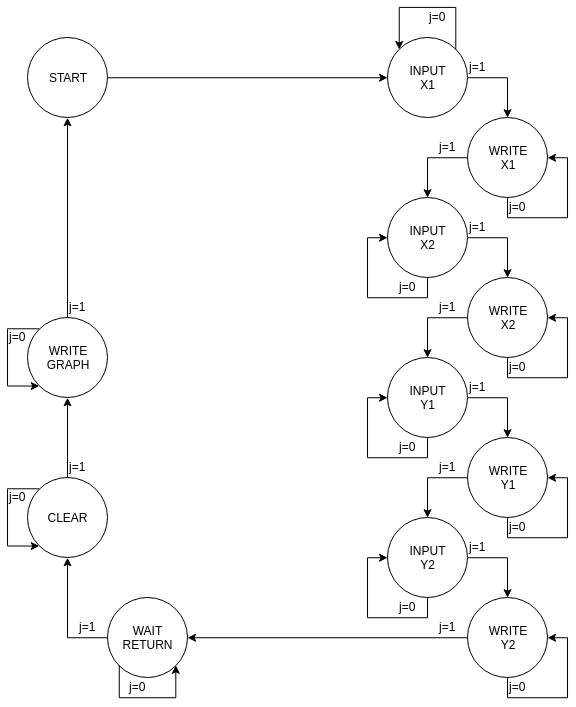
\includegraphics[width=\textwidth]{sm-vga}
        \caption{Máquina de Estados - Monitor}
        \label{fig:sm-vga}
    \end{figure}


O monitor usa uma máquina de estados [vga main fsm.vhd] que está sincronizado com a borda de descida de um clock de 10Hz.
Pois 50MHz era muito rápido para a transição de estados.

A máquina começa no estado [START], assim como o [COMEÇAR] da máquina de estados da regressão linear, 
passando para o [INPUTX1], que espera o input numérico do teclado para armazenar o valor e ligar a flag, passando para o estado [WRITEX1], 
que desenha o número na tela, na posição correta, os próximos [INPUT]'s e [WRITE]'s fazem a mesma coisa, mas para variáveis e posições
diferentes.

$$ x = 10 * X1 + X2 $$
$$ y = 10 * Y1 + Y2 $$

Assim que escritos X1, X2, Y1 e Y2, o estado [WAIT RETURN] irá esperar o usuário pressionar Enter, para limpara a tela em [CLEAR] e desenhar
o gráfico em [WRITE GRAPH], iterando 100 vezes incrementando o valor de x, e calculando o valor de y.

$$ x = x + 1 $$
$$ y = \theta_0 + \theta_1 * x $$

